%\chapter{Design of a SNP genotyping array specific to the African continent}
\section{Simulated and preliminary design of a SNP genotyping array specific to the African continent}
\label{sec:chip_design}

\subsection{Introduction}
As shown in table \ref{tab:chip_SNPs} on \pageref{tab:chip_SNPs), figure \ref{fig:SN02f2} and elsewhere\cite{Gurdasani2015} approximately 20\% of the autosomal SNPs on the Illumina HumanOmni2.5 SNP array are monomorphic in African populations. And as shown in figure \ref{fig:SN10f2} on page \pageref{fig:SN10f2} SNP density also alters imputation accuracy quite significantly. Therefore we wish to explore whether a continent specific array can capture variation in African populations better.

\begin{figure}
\centering
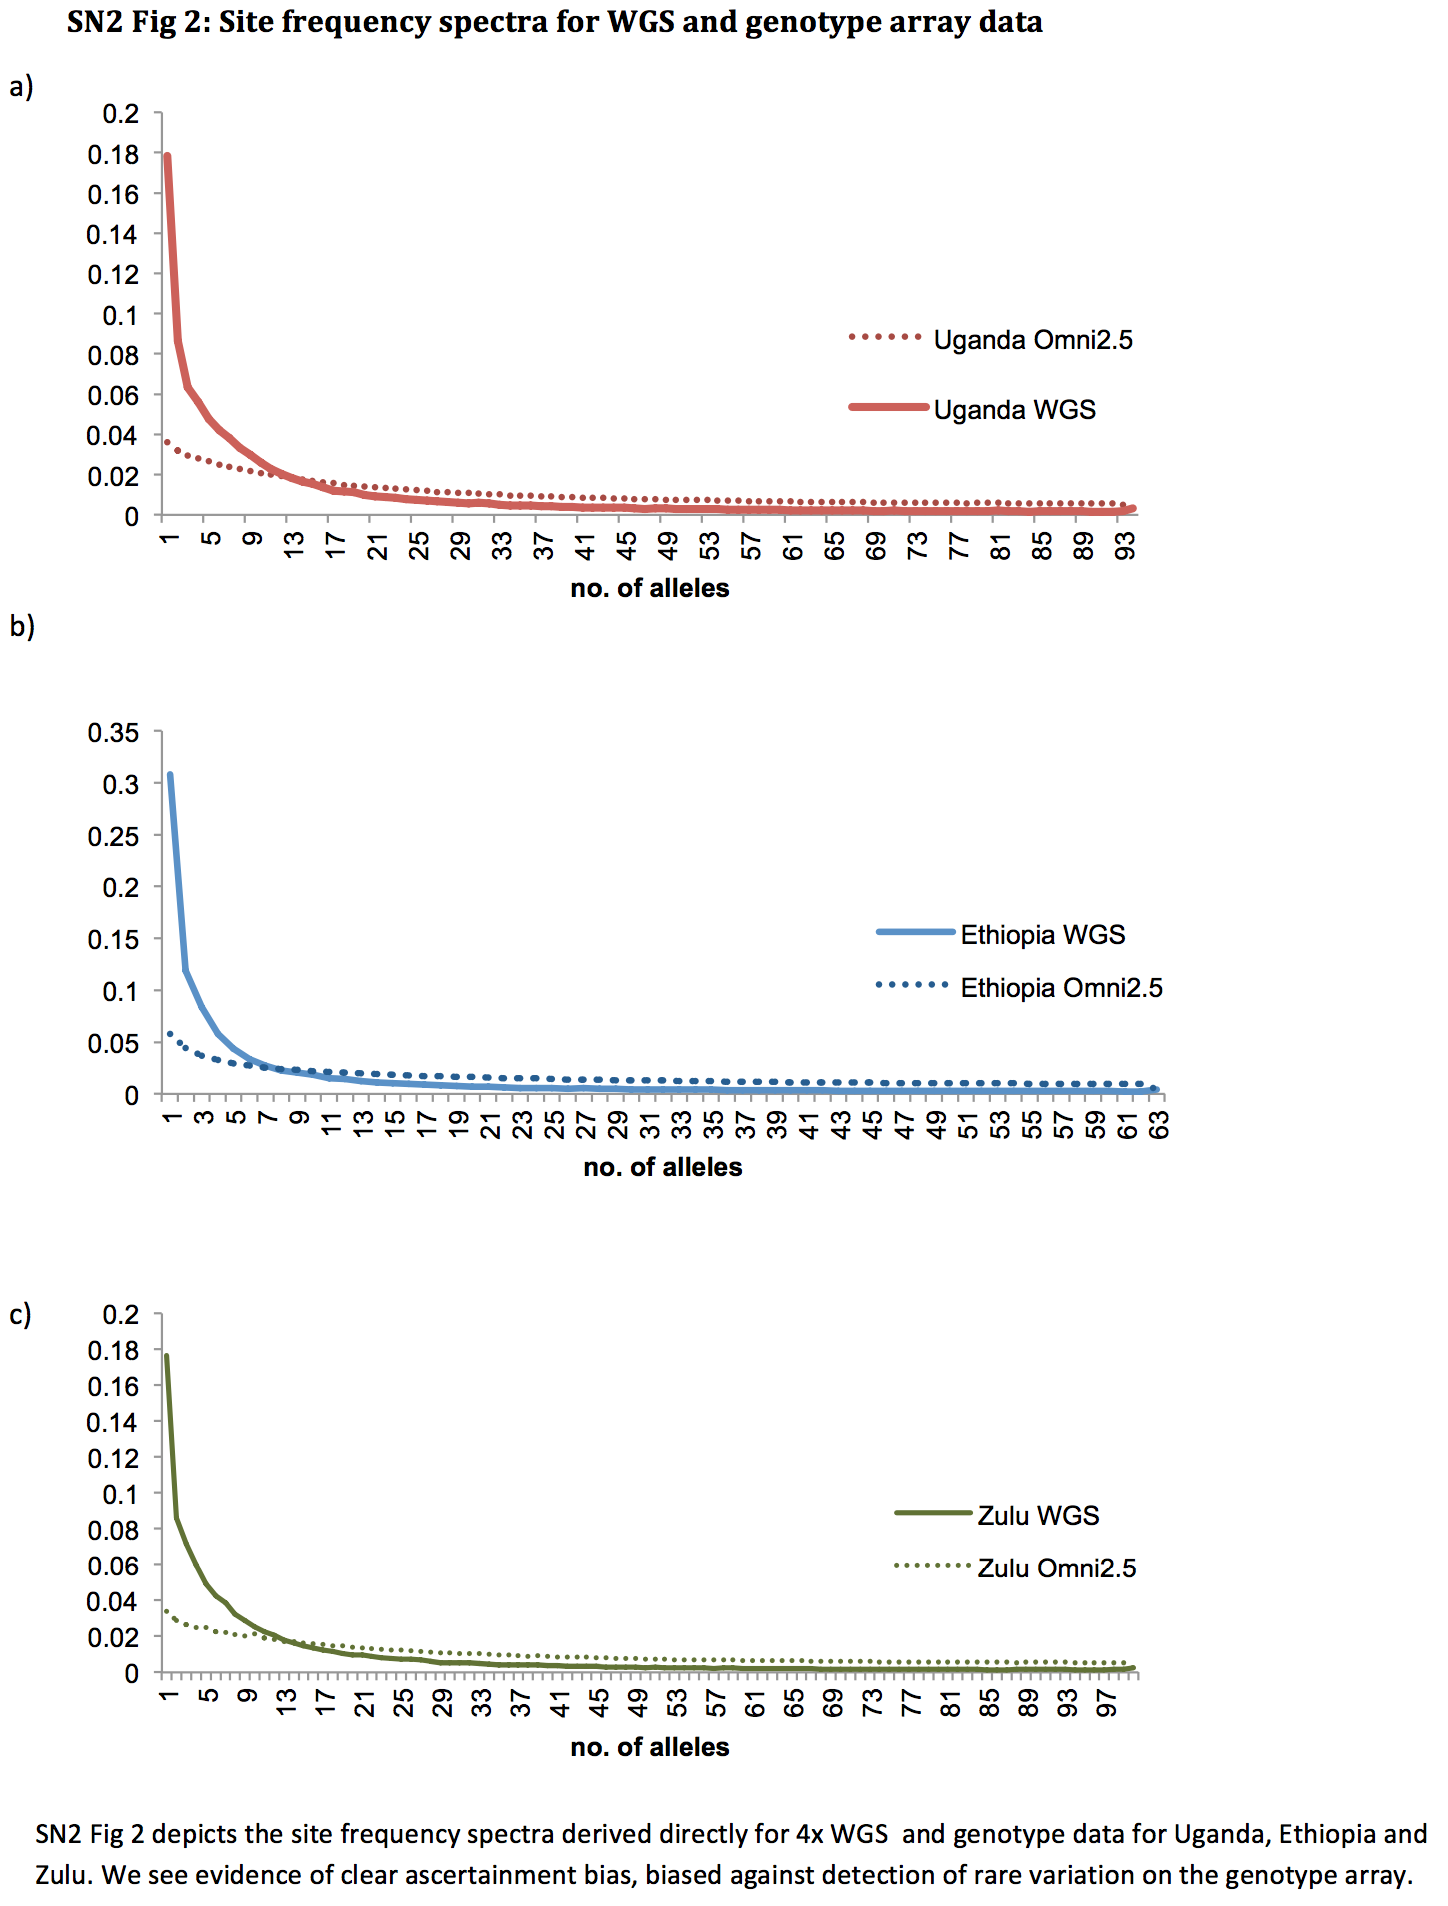
\includegraphics[trim={0 2cm 4cm 1cm},clip,width=0.8\textwidth]{fig/SN02f2}
\caption[Site frequency spectrum of sequence and SNP array data]{Site frequency spectrum derived directly from 4x \gls{WGS} data and SNP array data for the populations Uganda, Zulu and Ethiopia. Ascertainment bias against detection of rare variation on the SNP array is seen. On the x-axis is the number of alleles. On the y-axis is the relative frequency for each allele count.}
\label{fig:SN02f2}
\end{figure}

\begin{figure}
\centering
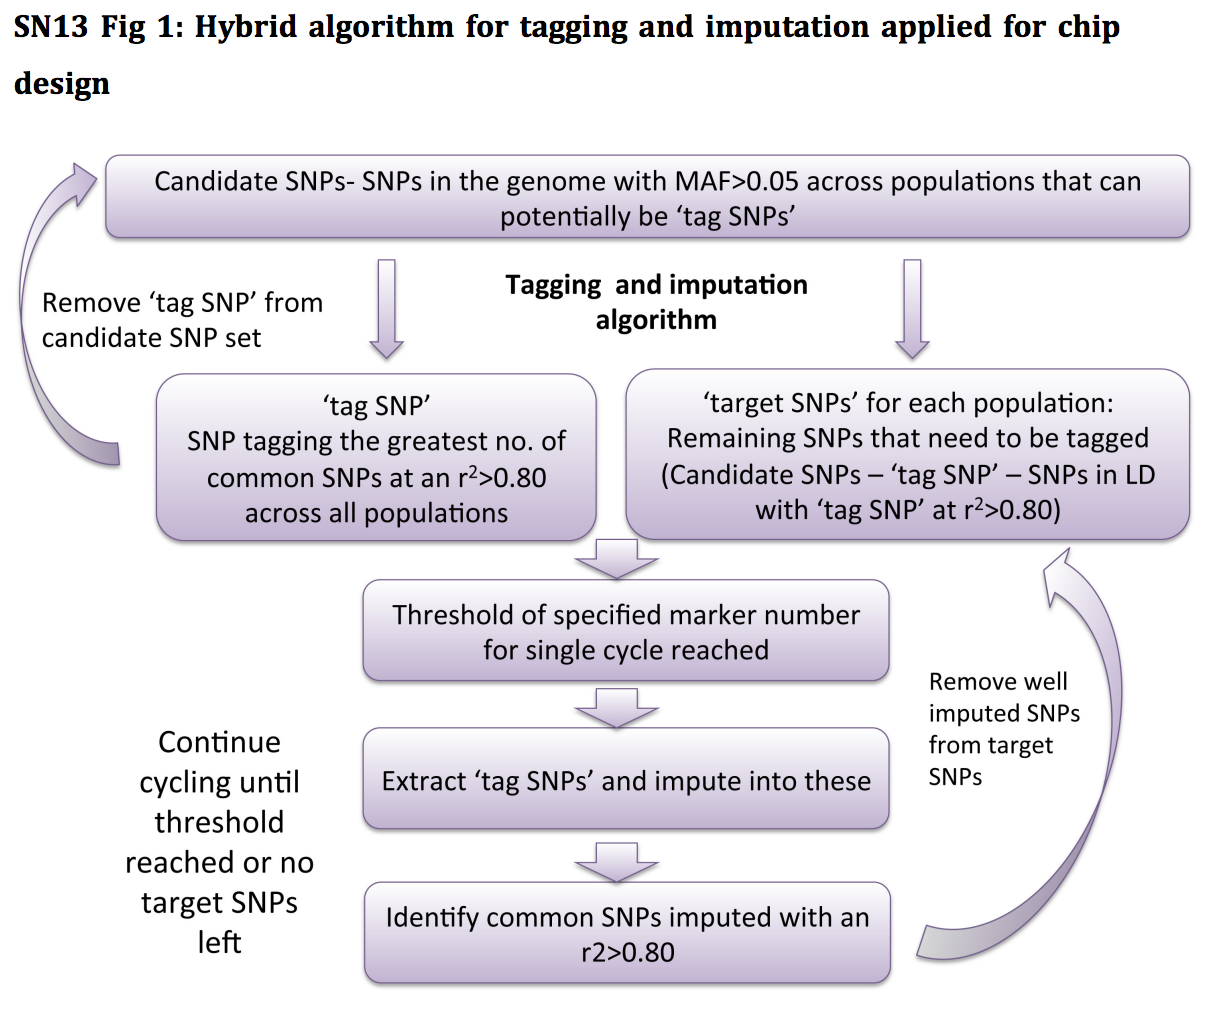
\includegraphics[trim={0 0 0 1cm},clip,width=0.75\textwidth]{fig/SN13f1}
\caption[xxx]{XXXXXXXX.}
\label{fig:SN13f1}
\end{figure}

\subsection{Data description}
\subsection{Methods}
Text
\subsubsection{Selection of tag SNPs}
\begin{figure}[htp]
\centering
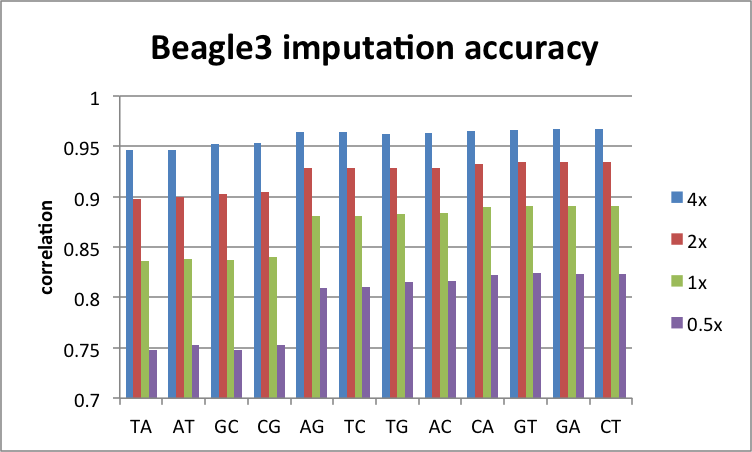
\includegraphics{Chapter3/fig/imp_accu_allele}
\caption{Imputation accuracy for each heterzygous allele. We used the Baganda 4x sequence data and SNP array data to calculate the genotype correlation for each heterozygous allele type. We found that the "mirror" alleles AT/TA and CG/GC for which it can be difficult to determine the relative strand have lower genotype correlations. }
\label{fig:imp_accu_allele}
\end{figure}

\paragraph{Greedy tag SNP Selection Algorithm}
\paragraph{Imputation with IMPUTE2}
\subsection{Results}
\subsubsection{Comparison of RagTagger with Existing Methods}
\subsubsection{Comparison of the Simple Greedy Algorithm and the Hybrid Algorithm}


\subsection{Discussion}
If more time and additional sequencing data had been available at the time of analysis, then it would have been interesting to compare the imputation accuracy, when using the Omni2.5M SNPs and the 1 million selected tag SNPs as an imputation scaffold. Given the large number of monomorphic SNPs on the Omni2.5M array and the European ascertainment bias, then it is expected, that the 1 million continent specific tag SNPs might perform better in terms of imputation accuracy.

\subsection{Conclusions}
